\section{State Charts}

\par
Due to the SPACS system being designed to be as stateless as possible, the only modules that have state diagrams are the Server and the Scheduler.

\subsection{Server}
\par
The Server is responsible for keeping the entire application running. In the event where part of the application dies, it will stop each part of the application then start it all back up, making sure that all these actions are logged.

\begin{figure}[!ht]
\begin{center}
	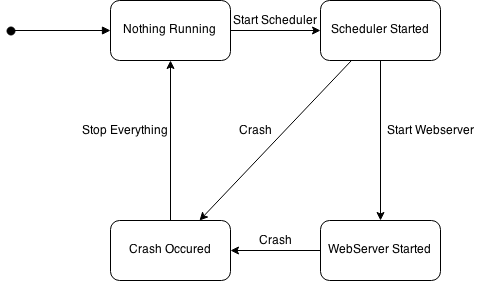
\includegraphics[width=10cm]{images/statechart_server}
	\caption{}
\end{center}
\end{figure}
\FloatBarrier

\subsection{Scheduler}
\par
The Scheduler manages all tasks that are supposed to run at fixed times or in fixed intervals. It will start up at a predetermined time and check for any jobs. If jobs exist, it will start processors for them and go back to idling. If no jobs exist it will just go straight back to idle.

\begin{figure}[!ht]
\begin{center}
	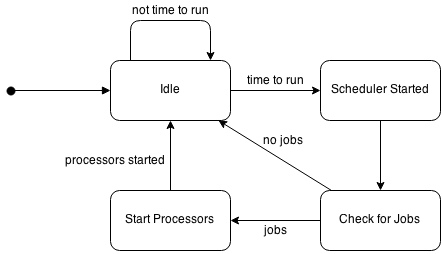
\includegraphics[width=10cm]{images/statechart_scheduler}
	\caption{}
\end{center}
\end{figure}
\FloatBarrier